\subsection{Neural Networks}

DNNs are trained by using a GMM-HMM to compute the maximum-likelihood
alignment of senones to frames, $s^{\ell,*}=\argmax
\pi(s_t^\ell,x^\ell|\theta)$, then minimizing the cross-entropy between
the senone sequence $s^\ell=[s_1^\ell,\ldots,s_T^\ell]$ and the neural
network output $y_{t}^\ell(s)=\Pr\left\{s_t^\ell=s\right\}$
(Fig.~\ref{fig:das1}).  The cross entropy is measured as
\begin{equation}
  H(S^\ell\Vert Y^\ell)=-\sum_{t=1}^T \sum_{s} \pi(s_t^\ell=s) \ln y_{s,t}^\ell
  \label{eq:dnn_train}
\end{equation}
A deterministic transcription contains no ambiguity in its phoneme
sequence; an unambiguous senone sequence can be computed using forced
alignment.  When $s_t^\ell$ is unambiguous, the gradient of
Eq.~\ref{eq:dnn_train} with respect to its model parameter matrix
($W$) is
\begin{equation}
  \nabla_W H(S^\ell\Vert Y^\ell)=-\sum_{t=1}^T
  \left(\frac{1}{y_t^\ell(s_t^\ell)}\right)\nabla_W y_t^\ell(s_t^\ell)
  \label{eq:dnn_dt}
\end{equation}
DNN training experiments were conducted in which the best path through
the PT, and the best alignment of the resulting senones to the
waveform, were both computed using forced alignment.  The resulting
best senone string was used to train a DNN using Eq.~\ref{eq:dnn_dt}.

\begin{figure}
  \centerline{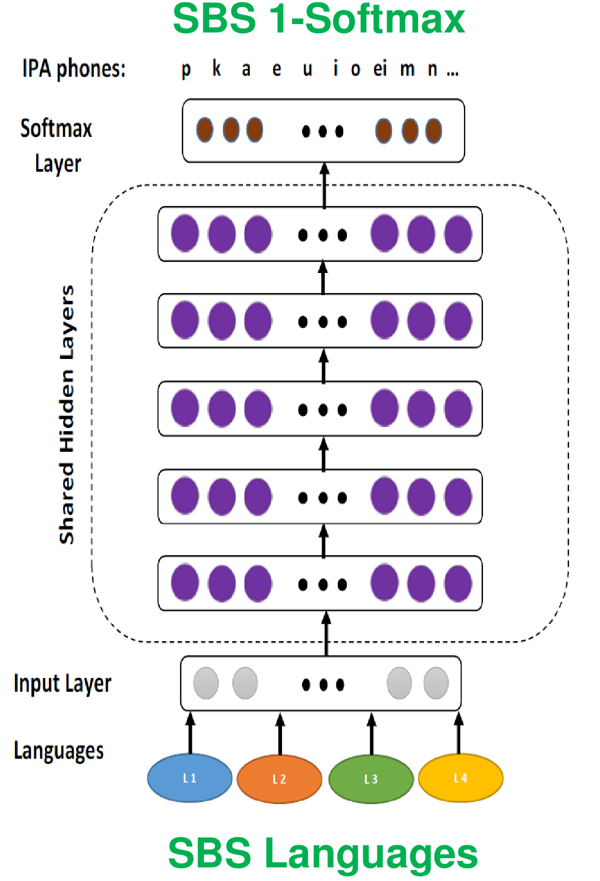
\includegraphics[width=2.5in]{../figs/das1.png}}
  \caption{Schematic of a deep neural network, showing a single
    softmax layer that computes the posterior probabilities of senones
    given knowledge of the acoustic features.}
  \label{fig:das1}
\end{figure}

